\documentclass[10pt,letterpaper]{article}
\usepackage{mathpazo}
\usepackage[scaled]{helvet}
\usepackage[T1]{fontenc}
\usepackage{hyperref}
\usepackage{color,soul}
\usepackage{graphicx}
\usepackage[justification=centering,singlelinecheck=false]{caption}
%\usepackage{setspace}
\usepackage[margin=1in,includehead,includefoot]{geometry}
\usepackage[table,dvipsnames]{xcolor}
\usepackage{amssymb}
\usepackage{amsmath}
\usepackage{fancyhdr}
\usepackage{array}
\usepackage{gensymb}
\usepackage{lastpage}
\usepackage{textcomp}
\usepackage{booktabs}
\usepackage{pdfpages}
\usepackage{tabto}
\usepackage{multicol}
\usepackage{tabularx}
\usepackage{framed}
\usepackage{chngcntr}
\usepackage{tocloft}
\usepackage[font={sf,normalsize},labelfont={sf,bf}]{caption}
\usepackage{float}
\usepackage{tikz}
\usepackage{listings}
\lstset{basicstyle=\small\ttfamily,breaklines=true}
\usepackage{forest}
\usepackage{verbatim}
\usepackage{longtable}
\usepackage{tabu}
\usepackage{afterpage}
\usepackage{paralist}
\usepackage{indentfirst}
\usepackage{changepage}

\newenvironment{Figure}
{\par\medskip\noindent\minipage{\linewidth}}
{\endminipage\par\medskip}

%% no indentation
%\setlength{\parindent}{0pt}

%%header and footer
\fancyhf{}
\renewcommand{\footrulewidth}{0pt}
\renewcommand{\headrulewidth}{0pt}
\rhead{\nouppercase{\leftmark}}
\lhead{\sf \textbf{Project 1}  |  Structure Learning}
\rfoot{\sf \textbf{0\thepage} OF \textbf{0\pageref*{LastPage}}}
\rhead{\sf \textbf{AA 228} | Decision Making Under Uncertainty}
\pagestyle{fancy}


%% DOCUMENT START --------------------------------------------------

\begin{document}
		
	\captionsetup[figure]{labelformat=simple, labelsep=quad, labelfont={sf, bf}}
	\captionsetup[table]{labelformat=simple, labelsep=quad, labelfont={sf, bf}}
	
	\section*{\sf \textbf{Bayesian Structure Learning}}
	\vspace*{-0.1 in}
	{\noindent \sf \large R. B. Alexander}
	
	\vspace*{0.2 in}
	
\begin{adjustwidth}{1cm}{1cm}
		
	\noindent \textbf{Bayesian structure learning is a combined structure learning and parameter learning task that involves learning the structure of a Bayesian network (a directed acyclic graph) $\mathbf{G}$ from a dataset $\mathbf D$. The dataset contains $\mathbf n$ discrete random variables $\mathbf X_{1:n}$. Each of the variables has $\mathbf r_i$ possible instantiations and for a given graph $\mathbf G$, each of the variables has $\mathbf q_i$ possible instantiations of its parents $\boldsymbol \pi_{ij}$. The number of times $\mathbf X_i = \mathbf k$ given $\boldsymbol\pi_{ij}$ occurs in the dataset is $\mathbf m_{ijk}$ and the associated probability of $\mathbf X_i = \mathbf k$ given $\boldsymbol\pi_{ij}$ is $\mathbf P(\mathbf X_i = \mathbf{k} \mid \boldsymbol\pi_{ij}) = \boldsymbol\theta_{ijk}$. Using the Bayesian score function, we can estimate the likelihood of a graph structure given the dataset. Once we have computed the Bayesian score, we must search the space of all Bayesian networks $\boldsymbol{\mathcal{G}}$ to find the graph that maximizes the Bayesian score and is thus, the most probable graph.}
	
\end{adjustwidth}
					
	\subsection*{\sf \textbf{Bayesian-Dirichlet Score Function}}
	
	For this project, the Bayesian-Dirichlet scoring function was used, which assumes a Dirichlet prior over the Bayesian network parameters ($P(\boldsymbol\theta) \sim \textnormal{Dir}(\boldsymbol\theta\mid\boldsymbol\alpha)$). The Bayesian-Dirichlet scoring function can be shown to take the following form, where $\Gamma$ is the gamma function, $\Gamma(n) = (n-1)!$.
	$$ \ln P(G \mid D) = \ln P(G) + \sum_{i=1}^n\sum_{j=1}^{q_i} \ln \left( \frac{\Gamma(\alpha_{ij0})}{\Gamma(\alpha_{ij0} + m_{ij0})} \right) + \sum_{k=1}^{r_i} \ln \left( \frac{\Gamma(\alpha_{ijk} + m_{ijk})}{\Gamma(\alpha_{ijk})} \right) $$
	with $\alpha_{ij0}$ and $m_{ij0}$ defined as:
	$$ \alpha_{ij0} = \sum_{k=1}^{r_i} \alpha_{ijk}$$
	$$ m_{ij0} = \sum_{k=1}^{r_i} m_{ijk} $$
	Since we have no information about which graph structures are more or less probable, we use a uniform graph prior, $P(G) = 1$. Under weak assumptions, we can assume a uniform Dirichlet prior over the Bayesian network parameters where $\alpha_{ijk} = \alpha$. Here, we set $\alpha = 1$, which gives the K2 scoring function:
	$$ \ln P(G \mid D) = \sum_{i=1}^n\sum_{j=1}^{q_i}\ln \Gamma(r_i) - \ln \Gamma(r_i + m_{ij0}) + \sum_{k=1}^{r_i} \ln \Gamma(1 + m_{ijk})$$
	
	\subsection*{\sf \textbf{Graph Search Algorithms}}
	
	The space of directed acyclic graphs is superexponential with the number of nodes, so an efficient search strategy is critical in finding an optimal Bayesian network. Several algorithms for graph search exist and two relevant classes of these algorithms are directed graph search algorithms and partially-directed graph search algorithms. Two prominent algorithms for directed graph search are K2 search, which greedily adds parents to a node until no higher-scoring graphs are found, and local search, which starts from a graph structure and moves to the highest-scoring graph in its neighborhood (defined by elementary graph operations). Algorithms for partially-directed graph search search the space of Markov equivalence classes, which is smaller than the space of directed graphs. Some algorithms exploit the \textit{score equivalence} of the scoring function to minimally search the space of partially-directed graphs, yielding robust searches.	
	
	\subsubsection*{\sf \textbf{K2 Search with Randomized Start}}
	
	The K2 search strategy begins from a completely unconnected graph. For a given node ordering $X_{1:n}$, the first node in the ordering $X_1$ is examined. An edge is added from one node in the exclusive node ordering $X_{1:n \backslash 1}$ to the examined node (for example, $X_2\to X_1$), the new graph is verified to be a directed acyclic graph, and the Bayesian score is computed. This process is repeated independently for each node in the exclusive node ordering after removing the previously added edge. Whichever of the new graphs gives the highest score is stored as the new best graph. The process repeats for the same examined node and parents are greedily added until none of the new graphs has a higher Bayesian score than the best graph. Then, this process is repeated by individually examining the next node in the node ordering $X_i$, and iteratively adding the parents from the new exclusive node ordering $X_{1:n\backslash i}$ until no improvement is made. Once the final node is examined and no improvements can be made, the K2 search is complete.
	
	\vspace*{0.1 in}
	
	It is clear that the node ordering strongly affects the final graph that is located in the K2 search. Since we have no information about which ordering is best, we assume a uniform distribution over possible node orderings. In our code, we set the seed of a random number generator for reproducibility and performed K2 searches on random permutations of node orderings. We theorize that a random search over K2 directed graph searches is likely to produce reasonable results much faster than a random directed graph search or a single deterministic K2 directed graph search. 
	
	\subsection*{\sf \textbf{Results}}
	
	In our implementation, we used K2 search and added randomized starts to identify several most-probable graphs, with one graph having the maximal Bayesian score. In particular, we examined three datasets: the \texttt{small} dataset, containing 8 variables; the \texttt{medium} dataset, containing 12 variables; and the \texttt{large} dataset containing 50 variables. The time for each search is provided in Table \ref{tab:runtime}.

	\begin{center}
		\captionof{table}{Runtimes in Seconds for K2 Search with Randomized Start}
		\vspace*{10pt}
		\label{tab:runtime}
		\begin{tabular}{l|l|l|l|l|}
			\cline{2-5}
			&                                                  \multicolumn{4}{c|}{\textbf{Iterations}}                                                   \\ \hline
			\multicolumn{1}{|l|}{\textbf{Dataset}} & \multicolumn{1}{c|}{\textit{1}} & \multicolumn{1}{c|}{\textit{10}} & \multicolumn{1}{c|}{\textit{100}} & \multicolumn{1}{c|}{\textit{1000}} \\ \hline
			\multicolumn{1}{|l|}{\texttt{small}}   & 3.1187                        & 16.341                         & 104.40                          & 1002.7                           \\ \hline
			\multicolumn{1}{|l|}{\texttt{medium}}  & 29.534                        & 249.30                         & 2516.8                          & \cellcolor[HTML]{EFEFEF}           \\ \hline
			\multicolumn{1}{|l|}{\texttt{large}}   & 8219.9                        & \cellcolor[HTML]{EFEFEF}         & \cellcolor[HTML]{EFEFEF}          & \cellcolor[HTML]{EFEFEF}           \\ \hline
		\end{tabular}
	\end{center}

	\vspace*{0.15 in}
	
	Since the $m_{ijk}$ counts only change marginally between graphs based on the assignment of new parents, it is possible to efficiently update only the necessary $m_{ijk}$ counts, leading to significant computational savings, especially on larger datasets. We did not implement efficient caching or recomputation of the counts, so the searches were quite computationally expensive. As a result, we limited the number of parents of any node to 8 to minimize the associated computational cost. It should be noted that in a K2 search, as parents are added, the Bayesian counts become more complex, but the total number of counts remains unchanged. At the same time, as more parents are added, the possibility of directed cycles increases and thus the space of valid Bayesian networks decreases, so the number of required computations tends to decrease as the search progresses. Figure \ref{fig:time_score_graph} shows the maximum Bayesian score and total search time as a function of the number of randomized search iterations. We observe only a marginal improvement in score with the logarithm of the number of iterations, but the computations scale linearly with time as expected. 
	
	\newpage
	
	\begin{figure*}[h!]
		\centering
		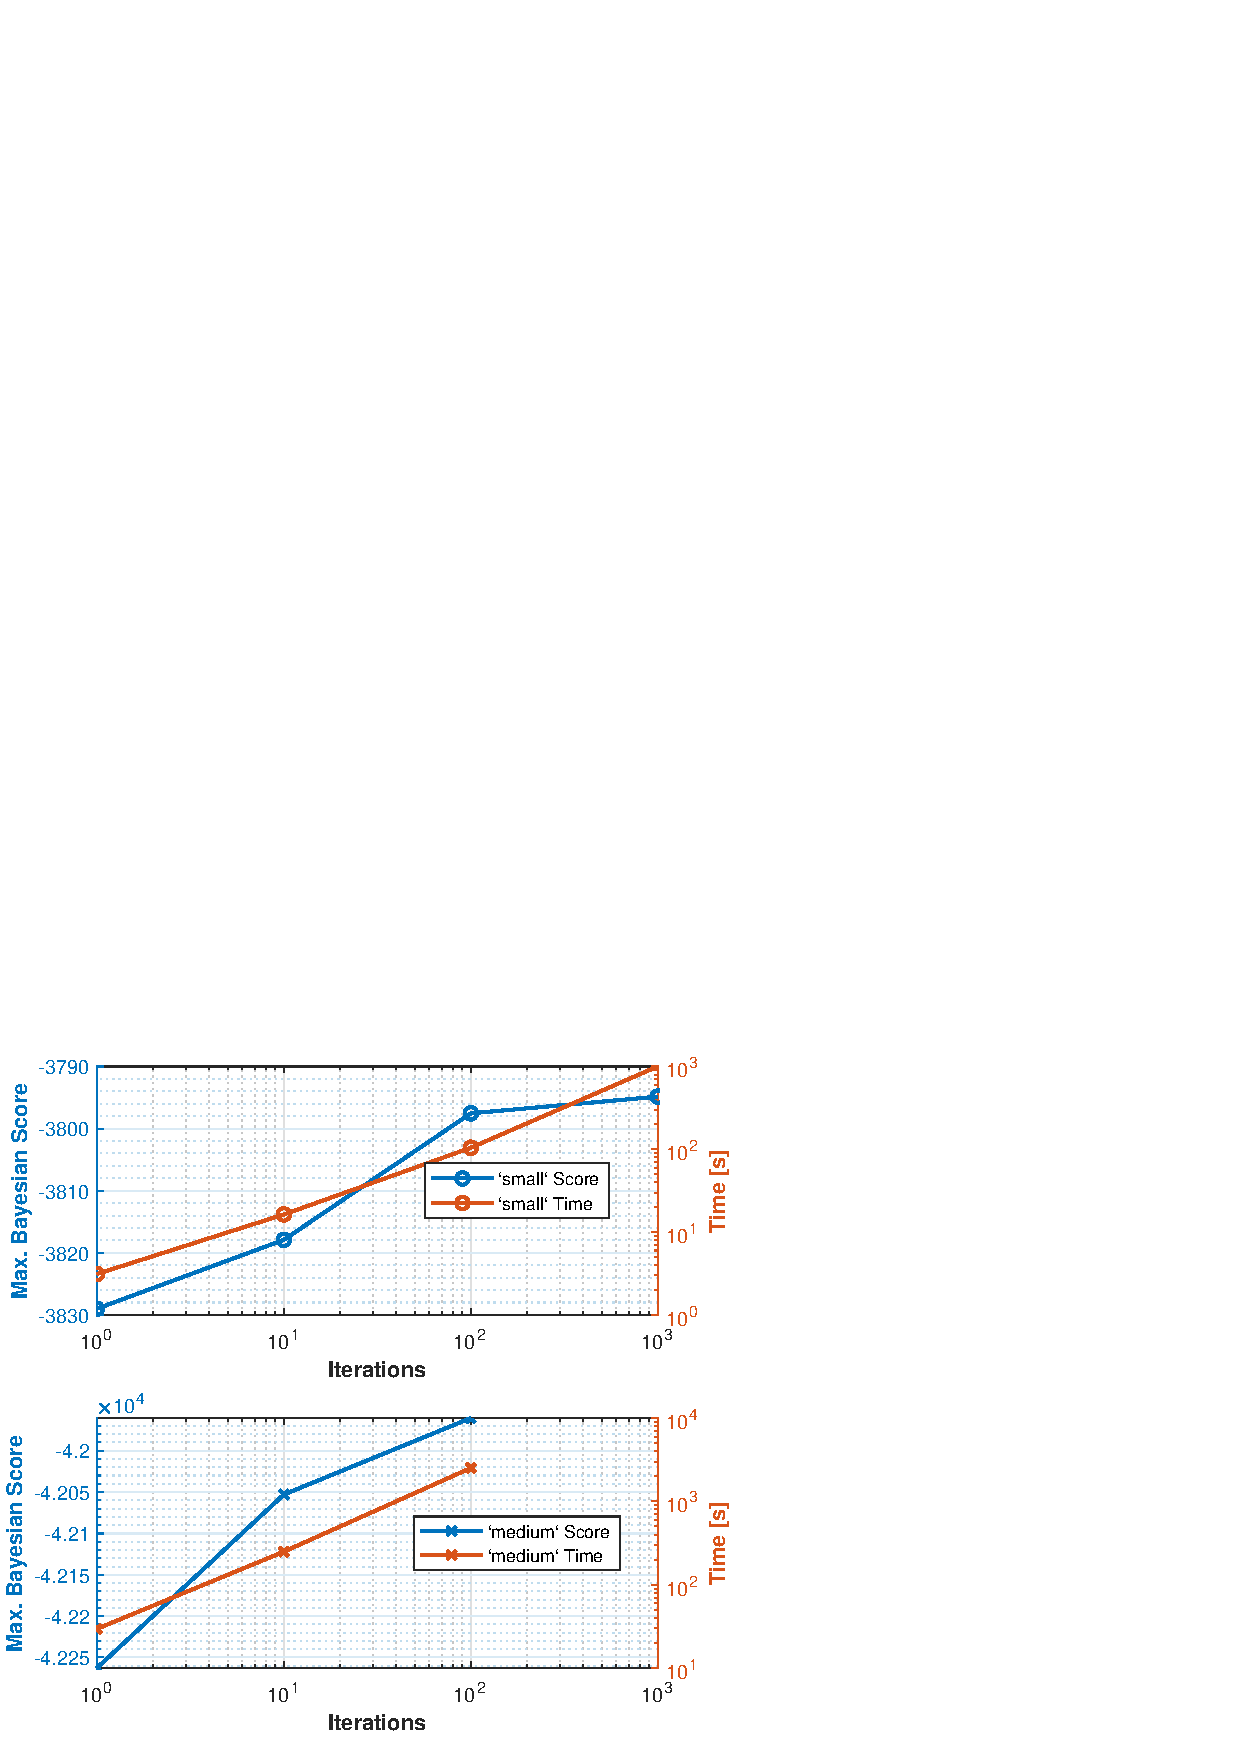
\includegraphics[width=0.47\linewidth]{figs/small-score-time.png}
		\hspace*{0.15 in}
		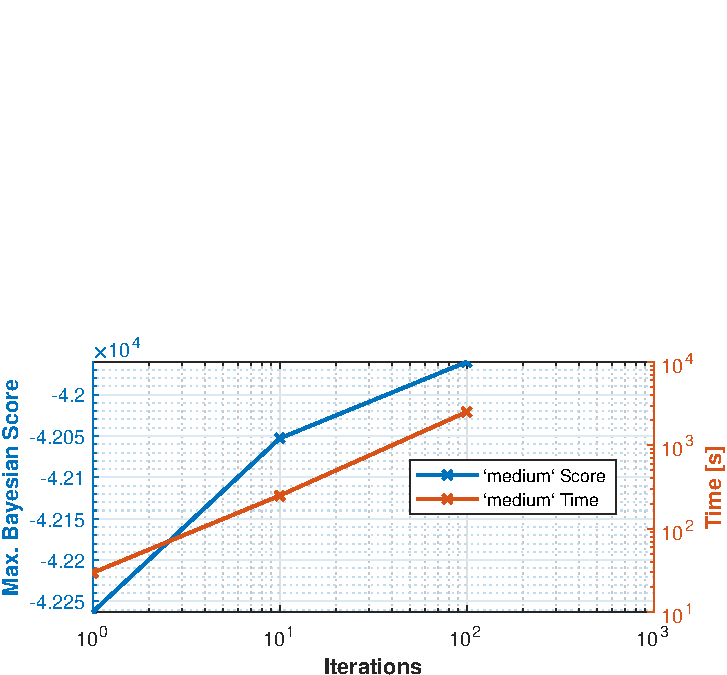
\includegraphics[width=0.47\linewidth]{figs/medium-score-time.png}
		\setlength{\belowcaptionskip}{-10pt}
		\captionof{figure}{Bayesian score improvement using K2 search iterated over randomly-permuted variable orderings for the \texttt{small} (\textit{left}) and \texttt{medium} (\textit{right}) datasets.}
		\label{fig:time_score_graph}
	\end{figure*}

	\vspace*{0.1 in}

\begin{multicols}{2}
	\begin{Figure} %[t]
		\centering
		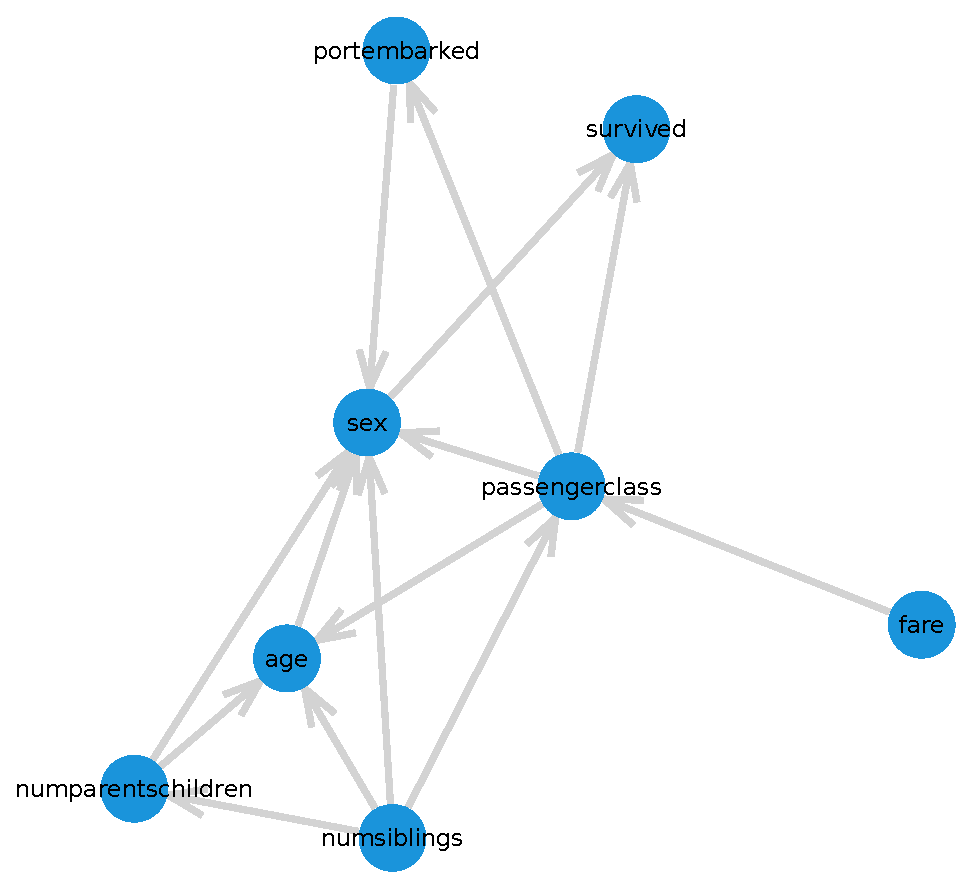
\includegraphics[height=0.33\textheight]{figs/small-K2-1000}
				\setlength{\belowcaptionskip}{-10pt}
		\captionof{figure}{\sf Bayesian network learned from the \texttt{small} dataset (8 variables) using a K2 search of the space of directed acyclic graphs with 1000 randomized starts. ($\ln P(G\mid D) \approx -3795 $)}
		\label{fig:small_graph}
	\end{Figure}
	\begin{Figure} %[t]
		\centering
		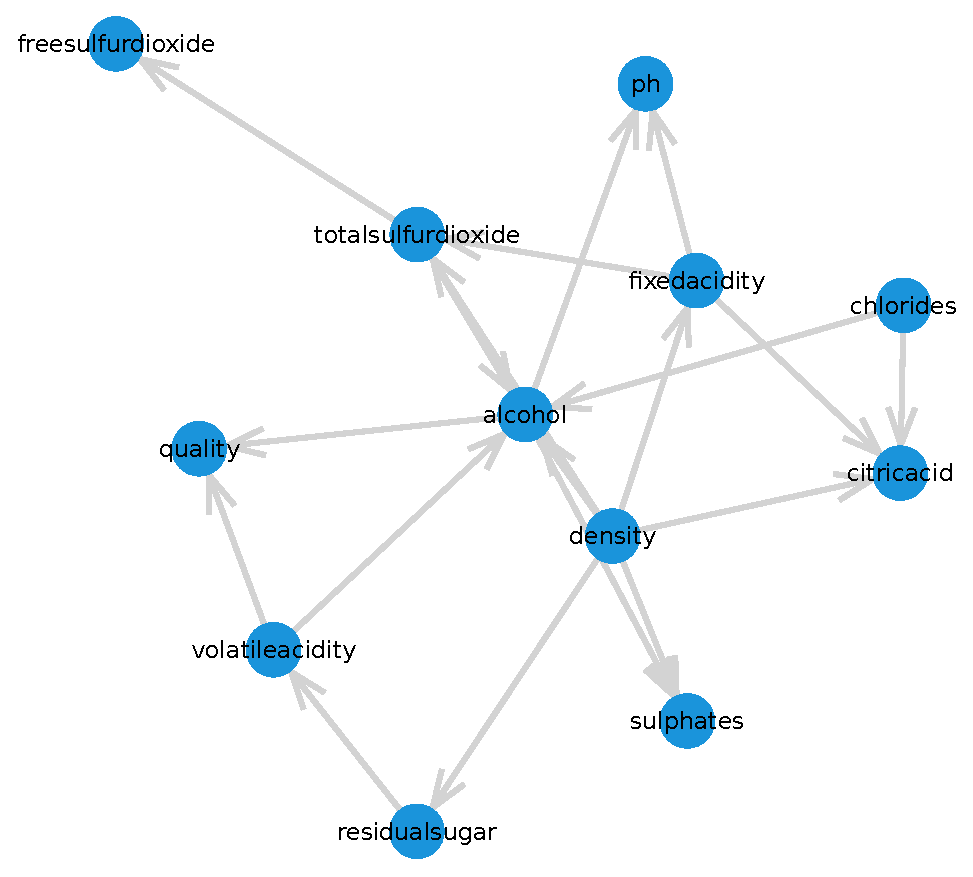
\includegraphics[height=0.33\textheight]{figs/medium-K2-100}
		\setlength{\belowcaptionskip}{-10pt}
		\captionof{figure}{Bayesian network learned from the \texttt{medium} dataset (12 variables) using a K2 search of the space of directed acyclic graphs with 100 randomized starts. ($\ln P(G\mid D) \approx -41961 $)}
		\label{fig:medium_graph}
	\end{Figure}
\end{multicols}

	\vspace*{0.1 in}
	
	The results of the graph searches produced the graphs displayed in Figures \ref{fig:small_graph}, \ref{fig:medium_graph}, and \ref{fig:large_graph}. In the \texttt{small} and \texttt{medium} graphs, we observe limited connectivity, whereas in the \texttt{large} graph, we can see a high degree of connection between the nodes. This demonstrates one of the core strengths of the Bayesian structure learning approach - \textbf{\textit{balancing model complexity with availability of data}}. 
	
	\vspace*{0.1 in}
	
	\textbf{In general, we were able implement a Bayesian structure learning framework with 1) a Bayesian scoring function and 2) directed graph search algorithms.}

	\begin{figure*}[h!] %[t]
		\centering
		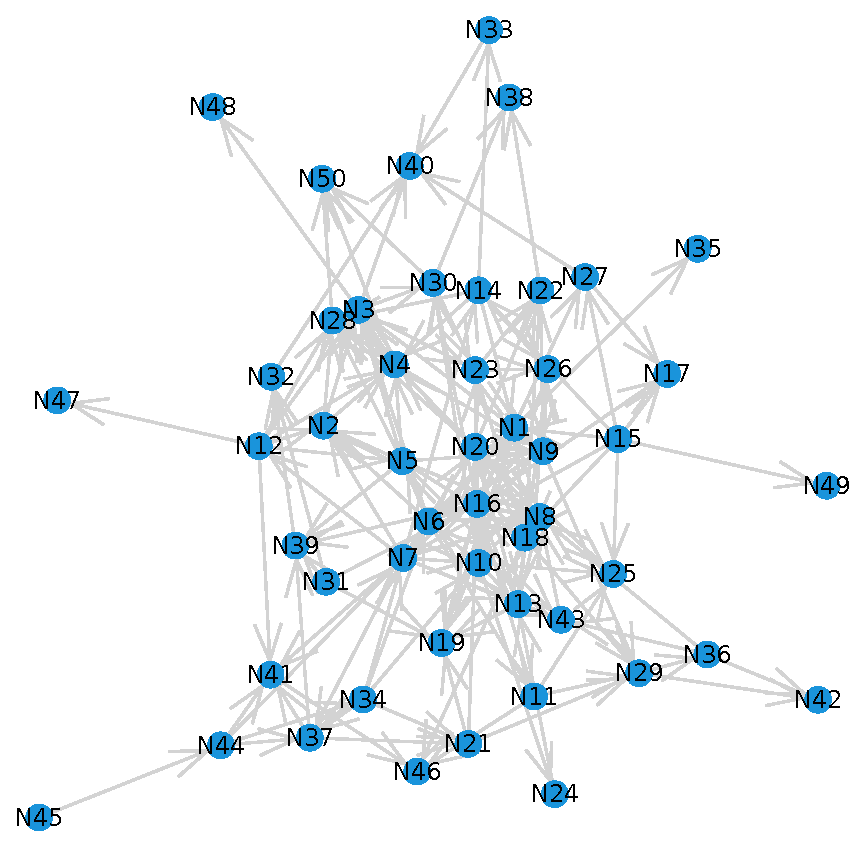
\includegraphics[height=0.8\textheight]{figs/large-K2-1}
		\setlength{\belowcaptionskip}{-10pt}
		\caption{Bayesian network learned from the \texttt{large} dataset (50 variables) using a K2 search of the space of directed acyclic graphs with 1 randomized start. ($\ln P(G\mid D) \approx - 427612$)}
		\label{fig:large_graph}
	\end{figure*}	
	
\end{document}